%% This is a skeleton file demonstrating the use of IEEEtran.cls (requires IEEEtran.cls version 1.8a or later) with an IEEE conference paper.
%%
%% Modified by Khan Reaz( kahn.reaz@ieee.org)
%% Support sites:
%% http://www.ieee.org/

%%***********************************************************
%% Legal Notice:
%% This code is offered as-is without any warranty either expressed or implied; without even the implied warranty of MERCHANTABILITY or FITNESS FOR A PARTICULAR PURPOSE!
%% User assumes all risk and can modify as s/he wants.

%%***********************************************************

\def\b0{{\bf 0}}
\def\ba{{\bf a}}
\def\bb{{\bf b}}
\def\bc{{\bf c}}
\def\bd{{\bf d}}
\def\be{{\bf e}}
\def\bg{{\bf g}}
\def\bh{{\bf h}}
\def\bi{{\bf i}}
\def\bj{{\bf j}}
\def\bk{{\bf k}}
\def\bl{{\bf l}}
\def\bm{{\bf m}}
\def\bn{{\bf n}}
\def\bo{{\bf o}}
\def\bp{{\bf p}}
\def\bq{{\bf q}}
\def\br{{\bf r}}
\def\bs{{\bf s}}
\def\bt{{\bf t}}
\def\bu{{\bf u}}
\def\bv{{\bf v}}
\def\bw{{\bf w}}
\def\bx{{\bf x}}
\def\by{{\bf y}}
\def\bz{{\bf z}}


\def\bSigma{{\bf \Sigma}}
\def\bA{{\bf A}}
\def\bB{{\bf B}}
\def\bC{{\bf C}}
\def\bD{{\bf D}}
\def\bE{{\bf E}}
\def\bF{{\bf F}}
\def\bG{{\bf G}}
\def\bH{{\bf H}}
\def\bI{{\bf I}}
\def\bJ{{\bf J}}
\def\bK{{\bf K}}
\def\bL{{\bf L}}
\def\bM{{\bf M}}
\def\bN{{\bf N}}
\def\bO{{\bf O}}
\def\bP{{\bf P}}
\def\bQ{{\bf Q}}
\def\bR{{\bf R}}
\def\bS{{\bf S}}
\def\bT{{\bf T}}
\def\bU{{\bf U}}
\def\bV{{\bf V}}
\def\bW{{\bf W}}
\def\bX{{\bf X}}
\def\bY{{\bf Y}}
\def\bZ{{\bf Z}}


%package list
\documentclass[conference]{IEEEtran}
\IEEEoverridecommandlockouts
\let\labelindent\relax
\usepackage{enumitem}
\usepackage{fleqn}
\usepackage{cite}
\usepackage{graphicx}
\usepackage[varg]{newtxmath}
\graphicspath{ {images/} }
\usepackage{pdfpages}
\usepackage{wrapfig}
\usepackage{fancyhdr}
\usepackage{lastpage}
\usepackage{lettrine}
\usepackage{amsmath}
% \usepackage{titlesec}
\usepackage[colorinlistoftodos]{todonotes}
\usepackage{float}
\usepackage[font={footnotesize}]{caption}
\usepackage[numbers,sort,square,compress]{natbib}
\usepackage[para]{footmisc}
\usepackage{xcolor}
\setlength{\belowcaptionskip}{-12pt}
\newcommand{\highlight}[1]{%
  \colorbox{red!50}{$\displaystyle#1$}}

% \usepackage{parskip}
% \setlength{\parskip}{0.02\baselineskip}

% \fancypagestyle{plain}{
%   \fancyhf{} % sets both header and footer to nothing
% \renewcommand{\headrulewidth}{0pt}
%   \fancyhead[C]{2018 International Conference on Indoor Positioning and Indoor Navigation (IPIN), 24-27 September 2018, Nantes, France}% Right header

% }
\pagestyle{plain}% Set page style to plain.

% \pagestyle{fancyplain}
% \fancyhf{}
% \renewcommand{\headrulewidth}{0pt}
% \fancyhead[C]{2018 International Conference on Indoor Positioning and Indoor Navigation (IPIN), 24-27 September 2018, Nantes, France}
\DeclareMathOperator*{\argmin}{argmin}
% \usepackage{titlesec}

% \titlespacing*{\section}{0pt}{1pt plus 2p}{1ex}
% \titleformat*{\section}{\fontsize{12}{12}\bfseries}
% \titleformat{\section}
%        {\normalfont\fontfamily{phv}\fontsize{12}{17}\bfseries}{\thesection}{1em}{}

% \titleformat{\subsection}
%        {\normalfont\fontfamily{phv}\fontsize{12}{17}\bfseries\itshape}{\thesubsection}{1em}{}

\begin{document}
%Here goes the title

\title{\vspace{-10pt}Predictive Quantization for MIMO-OFDM SVD Precoders using Reservoir Computing Framework \vspace{-10pt}}


%Authors List

 \author{\authorblockN{Agrim Gupta, Pranav Sankhe, Kumar Appaiah, Manoj Gopalkrishnan}
 \
 \authorblockA{Department of Electrical Engineering, Indian Institute of Technology Bombay\\
 \{agrim,pranavs,akumar,manojg\}@ee.iitb.ac.in \vspace{-18pt}}
% \thanks{Parts of this work was supported by the Bharti Centre for Communication in
% IIT Bombay, and the Visvesvaraya
% PhD Scheme of Ministry of Electronics \& Information Technology,
% Government of India (implemented by the Digital India Corporation).
% }}
}
\maketitle

\thispagestyle{plain}
%Main body starts



  % \noindent We consider problem of quantization and interpolation of
  % time and frequency varying precoding matrices in wireless MIMO
  % systems. Knowledge of precoder matrices at the transmitter can We first establish a result comparing the performance of
  % quantization and interpolation attempted directly over the Stiefel
  % manifold rather than over the Unitary manifold, as has been the
  % primary approach thus far. We propose a predictive quantization
  % algorithm to improve upon the quantization metric by exploiting both
  % time and frequency correlations in a constructed frequency hopping
  % scenario. Building upon these, we finally propose a joint
  % time-frequency interpolating algorithm to estimate the precoders
  % which were not fed back. We demonstrate significant improvements in
  % both BER curve and log-sum rate capacity over the existing
  % approaches.

\begin{abstract}

  % Precoding transmissions in wireless MIMO systems is essential to
  % enable optimal utilization of the spatial degrees of
  % freedom. However, communicating the precoding matrices from the
  % receiver is challenging, owing to large feedback requirements. Past
  % work has shown that predictive quantization in time, as well as
  % interpolation over frequency can be used to reconstruct the
  % precoders over a wide band, although these techniques have not been
  % used jointly. We propose both a predictive quantization as well as a
  % joint time-frequency interpolation strategy for precoding matrices
  % over the Stiefel manifold. The key insight that we use is that
  % local tangent spaces in the manifold permit effective combination of
  % both temporal and frequency domain information for more accurate
  % precoder reconstruction. Simulations reveal that we obtain a
  % significant improvement in achievable rate as well as BER reduction
  % when compared to existing strategies.

  Precoding in MIMO wireless systems is essential for achieving
  channel capacity. However, the receiver should quantize and feed
  back the precoder using very few bits of overhead. The precoder's
  underlying manifold structure aids this feedback and allows the use
  of channel temporal/frequency correlation for predictive
  quantization. We introduce a reservoir computing framework for
  predictive quantization by exploiting temporal correlations. Past
  methods primarily use the geometry of the underlying manifold for
  precoder prediction.  We, instead, use a dynamical reservoir state
  as part of the online training process of the reservoir.
  Simulations reveal reduces quantization error, lower BER and
  improved achievable rates.
\end{abstract}


\vspace{-5pt}
\section{Introduction}
\label{intro}
% Broad summary of your work, come to your problem definition.
% Can remove MIMO wireless systems
In MIMO wireless systems, precoding matrices are used to transform of an $N_S$-dimensional ($N_S \leq \text{min}(N_T,N_R))$ data stream onto an $N_T$-dimensional transmit signal.
The precoding matrix used to maximize the achievable rate using optimal power allocation is obtained via the SVD of the MIMO channel matrix \cite{love2008overview}.
However, since the MIMO channel matrix is estimated at the receiver, the transmitter requires receiver feedback for optimal precoding.
Therefore, the receiver needs to quantize and feed back the precoders while respecting the bit budget imposed by limited feedback schemes.
Given the high dimensionality of precoders (which form a $N_T \times N_R$ complex-valued matrix, viz. $2N_TN_R$ real numbers), effective quantization with just a few bits poses a significant challenge.

% Elaborate on each point (what people have done before) lecunnas
Past work has used two inherent properties of the optimal precoders to enable effective quantization with just a few bits.
First, the optimum precoders are not actually $2N_TN_R$ dimensional entities, but have an underlying manifold structure that allows to work with effective lower dimensions, when performing operations over the manifold directly \cite{pitaval2013codebooks}.
Second, these precoders are correlated in both time and frequency \cite{Gupt1905:Predictive}.
Utilizing the available correlations permit the use of predictive quantization algorithms, which enable improvement of the quantization error with time.
This improvement is obtained because of feeding back just the small extra information needed on top of the past fed back precoders, as compared to the new precoder information in the entirety.
% Exploiting frequency correlations permits the use of interpolation algorithms, which reduce the feedback overhead in a single OFDM frame, by feeding back CSI only for certain subcarriers, and interpolating over the others.

Combining the two inherent properties (viz. manifold structure and correlations) to frame manifold based predictive quantization algorithms, require a generalization of various well known linear algorithms for prediction, quantization and interpolation, to the underlying non-linear manifold structure. This is typically done by exploiting the differential geometry of the manifold and relevant past work in this direction has been presented in \cite{Gupt1905:Predictive,6891198,6545375,5671092,Li2016,krishnamachari2013geometry,chang2011adaptive}. Manifold based approaches for predictive quantization have provided significant performance benefits, given that they work with the effective lower dimensions while framing the manifold operations to predict and quantize.
However, these approaches are non-trivial, since they require specific operations over the non-linear manifold differential geometry.
In this paper, we aim to capture the above non-linear relations using a reservoir computing based predictive quantizer to exploit the temporal correlations effectively.
The proposed framework offers a simple solution to the predictive quantization problem, which brings about ease of implementation, along with improved performance, when compared to \cite{6891198}, which proposed a corresponding manifold based method to the problem considered in this paper.

% How to we do this
%\textcolor{blue}
{
Reservoir computing (RC) is a computational framework designed for sequential data processing.
% Its design is inspired from several frameworks of Recurrent Neural Networks \cite{jaeger2004harnessing}, including Liquid State Machines \cite{jalalvand2015real} and Echo State Networks \cite{mosleh2017brain,pathak2017using}.
The RC framework represents the non-linear relationships in the data via the higher dimensional dynamical reservoir state vector, which is transformed (using matrices, referred to as `couplers') to the lower dimensional input/output vectors. The couplers are learnt over time to map the transformations from reservoir state to the output, optimally.
% A reservoir computing system maps the inputs to temporal patterns in a higher dimensional dynamical reservoir state.
% The pattern analysis over these temporal patterns is performed by an output coupler that maps the higher dimensional reservoir state back to the output dimension that generally possesses lower dimensionality than the reservoir state.
% A important characteristic of reservoir computing is that while training, the input weights and the weights within the reservoir are not kept fixed and the weights of the output coupler are updated.
% Key advantages of reservoir computing framework include ease of training in comparison to its counterparts like Deep Neural Networks \cite{mosleh2017brain}.
RC has been successfully used to solve problems like handwritten digit image recognition \cite{jalalvand2015real}, climate prediction \cite{pathak2017using}, as well as problems in the domain of wireless communications \cite{jaeger2004harnessing,mosleh2017brain,shafin2018realizing}.
\cite{jaeger2004harnessing} used RC framework to harness channel non-linearities for improved channel equalization.
\cite{mosleh2017brain,shafin2018realizing} utilized the framework for OFDM symbol detection while accounting for channel and power amplifier non-linearities.
In our work, we utilize a RC framework to capture the underlying nonlinear relations between the previously fed back precoders and the precoder at next time instant, for predictive quantization. This becomes analogous to time series prediction algorithms, for which the RC framework has been cited to work effectively \cite{mosleh2017brain}.

\vspace{-1pt}
\section{System Model}
\label{section2}

We consider a $N_T\times N_R$ MIMO-OFDM wireless system with $N$ subcarriers, and assume $N_T > N_R$ and $N_s = N_R$.
Consistent with notation in \cite{6891198,Gupt1905:Predictive}, the data stream received on the $i$-th subcarrier, $t$-th time instant (or the $t$-th OFDM frame) is,
\vspace{-1pt}
\begin{equation}
\by_{i,t}=\bH^{H}_{i,t}\tilde{\bU}_{i,t}\bx_{i,t}+ \bw_{i,t}
\end{equation}
\vspace{-1pt}
Here, $\tilde{\bU}_{i,t} \in \mathbb{C}^{N_T \times N_R}$ is the quantized estimate of precoding matrix, $\by_{i,t} \in \mathbb{C}^{N_R \times 1}$ is the received data stream, $\bx_{i,t} \in \mathbb{C}^{N_T \times 1}$ denotes the transmitted signal, $\bH_{i,t} \in \mathbb{C}^{N_T \times N_R}$ denotes the point-to-point MIMO channel matrix and $\bw_{i,t}$ denotes the i.i.d. complex Gaussian noise with $\bw_{i,t} \sim \mathcal{N}_{\mathbb{C}}(0,N_0\bI_{N_R})$, $N_0$ being the noise variance. For this work, we assume that $\bH^{H}_{i,t}$ is estimated exactly, with zero error at the receiver.

% Tell that if infinite bit budget available, transmitter can directly use matrices obtained from SVD as precoders. However, since this is not the case we have to quantize (N dimensional) manifold, incurring substantial quantization error. Independent quantization techniques (references). Predictive quantization techniques can be used on the top of independently initialized values to improve the error. This is done in a way intuitively similar to Delta PCM, in which quantization error is reduced substanitally by using a linear predictor and quantizing the difference between the predicted and observed value. Since these preocders lie on Stiefel manifold, linear schemes will not work, due to non linearity of the manifold. However,past work has generalized the ideas to the manifold by exploiting the differential geometry of the manifold. Once a prediction is obtained, one has to quantize only the difference between the prediction and the observed value, which allows for improved quantization error. As the prediction becomes closer to the original value, the quantization error also decreases. The quantization algorithm is illustrated in Section 3.3


Given infinite bit budget, the transmitter can directly use the matrices obtained from SVD of $\bH^{H}_{i,t}$ as the precoder $\tilde{\bU}_{i,t}$.
That is, if $\text{SVD}(\bH_{i,t}) = \bU_{i,t},\Sigma_{i,t}, \bV_{i,t}$, then $\tilde{\bU}_{i,t} = \bU_{i,t}$.
The matrices $\bU_{i,t}$ reside on the Stiefel manifold $\text{St}(N_T,N_R)$, since the columns of $\bU_{i,t}$ form a set of $N_R$ orthogonal vectors in $N_T$ dimensions \cite{Gupt1905:Predictive,6891198}.
Given practical limitations, only limited feedback is available from the receiver, and the objective is to estimate $\bU_{i,t}$, via $\tilde{\bU}_{i,t}$, using the available feedback bits. Independent quantization algorithms analogous to the Lloyd codebook algorithm have been studied for quantizing the complete $\text{St}(N_T,N_R)$ \cite{6678348}.
However, this approach treats precoders close to each other in time/frequency as independent, since it does not exploit any temporal/frequency correlations.

Predictive quantization algorithms \cite{Gupt1905:Predictive,6891198} can be utilized to reduce the quantization error by utilizing correlations.
We now discuss the basic mathematical model that is central to predictive quantization algorithms for precoding matrices.
Suppose that we predict the current precoding matrix based on the past $p$ observed precoding matrices. For this, assume that $\tilde{\bU}_{i,t-p},\ldots,\tilde{\bU}_{i,t-1}$ have been fed back to the transmitter.
By using a prediction algorithm to exploit the time correlations among precoders at time instances $t-p,\ldots,t-1$, the transmitter can obtain a prediction (viz. a coarse estimate) of $\bU_{i,t}$, given by $\bP_{i,t}=f_P(\tilde{\bU}_{i,t-p},\ldots,\tilde{\bU}_{i,t-1})$, where $f_P(\cdot)$ is a prediction function.
Now, since the transmitter already possesses a coarse estimate $\bP_{i,t}$ of $\bU_{i,t}$, the receiver just quantizes the local space of $\text{St}(N_T,N_R)$ nearby $\bP_{i,t}$. The receiver feeds back this quantized information, enabling a refined estimate of $\bU_{i,t}$, given by $\tilde{\bU}_{i,t}$.
That is, the transmitter utilizes a quantization function $q_P(\cdot)$, to obtain $\tilde{\bU}_{i,t} \gets q_P(\bP_{i,t},\text{fb}_{i,t})$, where $\text{fb}_{i,t} \in \{1,2\ldots2^{\mathcal{B}}\}$ is feedback for the precoder at $i$-th subcarrier, $t$-th time instant, considering bit budget of $\mathcal{B}$ bits.
In \cite{Gupt1905:Predictive,6891198,6545375}, $\text{fb}_{i,t}$ denotes the codeword index for the codebook obtained by quantizing the local tangent space at $\bP_{i,t}$.

% When using the predictive quantization scheme, the quantization is performed on a smaller subspace when compared to the entire manifold in case of independent quantization.
% Therefore, the quantization error is substantially lower as well.
% However, independent quantization algorithms are important for smart initialization (instead of a cold start) of the predictive quantization strategies.
% Observe that predictive quantization algorithms for SVD precoders are typically the higher dimensional analogues of well known approaches to reduce quantization error using linear prediction codes (LPCs) and Delta PCM.
% In both LPCs and Delta PCM, quantization error can be reduced substantially using a linear predictor and quantizing the scalar difference between the predicted and observed value (innovation).
% Analogous to this, for $\text{St}(N_T,N_R)$, quantization error is reduced by quantizing a subspace around the predicted value that is much smaller than the entire manifold. In our work, we propose a RC framework which implements the prediction function $f_p(\cdot)$.
We reuse the $q_P$ algorithm from \cite{Gupt1905:Predictive,6891198}.
However, by incorporating the $q_P$ in the reservoir framework, $f_P$ and $q_P$ get coupled in the sense that $f_P$ is optimized via online training of the reservoir by minimizing the norm difference between $\bP_{i,t}=f_P(\cdot)$, and $\tilde{\bU}_{i,t}=q_P(f_P(\cdot),\text{fb}_{i,t})$.
Previous work \cite{Gupt1905:Predictive,6891198} has considered $f_P$ and $q_P$ to be uncoupled with each other.
% A detailed discussion on the RC based model for $f_P$ and $q_P$ is presented in Section \ref{section3}.
% The proposed RC scheme is evaluated against the temporal predictive quantization scheme in \cite{6891198}, and the simulation results are discussed in Section \ref{section4}.

%Explain prediction and quantization steps here itself ! (succintly)
\section{Reservoir Framework for Pred. Qtizn.}
\label{section3}
% \subsection{Vectorizing matrices in the Stiefel Manifold}
% \label{vectorize}
The RC framework has inputs and outputs as real vectors, and thus, it is necessary to convert the precoding matrices to vectors.
A precoding matrix $\mathcal{\bM} \in \text{St}(N_T,N_R)$ is a $\mathbb{C}^{N_T \times N_R}$ matrix with the property $\mathcal{\bM}^H\mathcal{\bM}=\text{\textbf{1}}_{N_R}$.
For brevity, we call such a matrix $\mathcal{\bM}$ a `semi-unitary' matrix.
A na{\"i}ve method to vectorize a $\mathbb{C}^{N_T \times N_R}$ semi-unitary matrix would be to take all its $N_TN_R$ complex numbers individually and stack them onto a $2N_TN_R$ dimensional real vector.
However, a more efficient approach would be to use the $\mathcal{\bM}^H\mathcal{\bM}=\text{\textbf{1}}_{N_R}$ property, which implies that each vector that represents the columns of $\mathcal{\bM}$ is orthogonal to the other columns.
For the first column, we take its $N_T$ complex numbers and stack them onto a $2N_T$ vector.
For the second column, we take only the first $N_T-1$ complex numbers and concatenate, since the last number can be determined by utilizing orthogonality with the first column.
For the third column, we take only the first $N_T-2$ complex numbers, and so on.
Therefore, we vectorize a $\mathbb{C}^{N_T \times N_R}$ semi-unitary matrix $\mathcal{\bM}$ into a $2(N_T)+2(N_T-1)+\ldots+2(N_T-N_R+1)= 2N_TN_R-N_R^2+N_R$ dimensional vector, denoted as $\bm$.

% Observe here that we incur a dimensional penalty upon vectorizing semi-unitary matrices.
% $\text{St}(N_T,N_R)$ is a $2N_TN_R-N_R^2$ dimensional manifold, whereas the proposed vectorization yields a $2N_TN_R-N_R^2+N_R$ dimensional vector representation.
% This corresponds to an overhead of $N_R$ dimensions, since we have not exploited the fact that each of the $N_R$ column vectors is a unit norm vector as well.
% It looks as if utilizing the norm 1 property, we could just take $N_T-1$ complex numbers when vectorizing the first column, instead of $N_T$. However, this would lead to non-unique representations, since there could then be infinite possible values that the lone missing complex number can take, so that the vector has unit norm.
 % Hence, we vectorize a semi-unitary $\mathbb{C}^{N_T \times N_R}$ $\mathcal{\bM}$ into $2N_TN_R-N_R^2+N_R$ dimensional vector, denoted as $\bm$.
%Focus on the fact that you don't actually pay a penalty
%The thing to quantize remains on the Stiefel Manifold
% \subsection{Forward Prediction $f_P$}

The input to the reservoir $i$ that corresponds to subcarrier $i$ is $\tilde{\bu}_{i,t-1}$ (vectorized representation of $\tilde{\bU}_{i,t-1}$), with dimensions $D_{\text{in}}=2N_TN_R-N_R^2+N_R$.
Using a randomly initialized $D_{\text{resv}}\times D_{\text{in}}$ input coupler matrix $\bW^{\text{in}}_i$, the $D_{\text{in}}$ dimensional input is mapped to a $D_{\text{resv}}(>>D_{\text{in}})$ dimensional vector, where $D_{\text{resv}}$ is the dimension of the reservoir state vector $\br_{i,t}$. $\br_{i,t}$ is initialized with $D_{\text{resv}}$ zeros, and is updated via the following equation:
\begin{equation}
\br_{i,t}=\text{tanh}(\bA_i\br_{i,t-1}+\bW^{\text{in}}_i\tilde{\bu}_{i,t-1})
\label{res_upd}
\end{equation}
where $\bA_i$ is the adjacency matrix that captures the reservoir dynamics, and $\text{tanh}$ is applied element wise.
Typical choices for $\bA_i$ have been Erdos-Renyi graphs with an upper bounded maximum eigenvalue \cite{mosleh2017brain,pathak2017using}. The output of the reservoir is $\bp_{i,t}$ (vectorized representation of $\bP_{i,t}$), which denotes the predicted precoder at $i$-th subcarrier, $t$-th time instant.
Therefore, the output of the reservoir is also a $D_{\text{in}}$ dimensional vector (viz. $D_{\text{out}}=D_{\text{in}}$).
The output $\bp_{i,t}$ is obtained using a matrix transformation of the reservoir state $\br_{i,t}$ with $D_{\text{out}}\times D_{\text{resv}}$ output coupler matrix $\bW^{\text{out}}_{i,t-1}$, which forms the prediction function $f_P(\cdot)$ with $\tilde{\bU}_{i,t-1}$ as its argument, for the RC framework
\begin{equation}
\bp_{i,t}=\bW^{\text{out}}_{i,t-1}\br_{i,t}=f_P(\tilde{\bU}_{i,t-1})
\label{pred_op}
\end{equation}

\begin{figure}[ht]
\centering
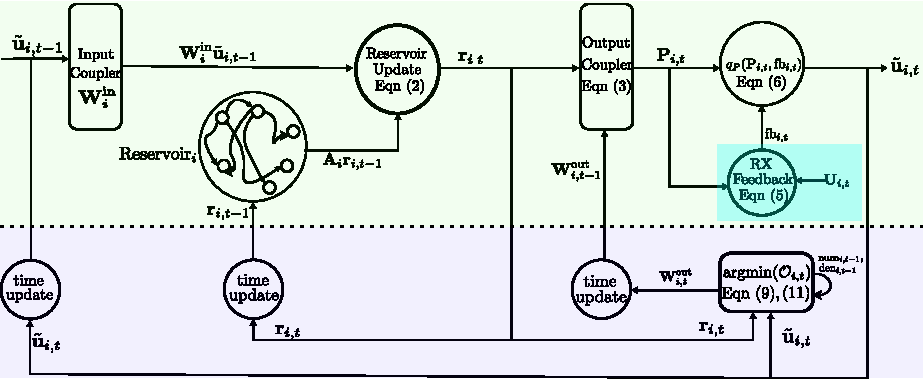
\includegraphics[width=0.5\textwidth]{images/system2.pdf}
% \caption{System Overview: The RC framework takes the precoder estimate at $t-1$ (viz. $\tilde{\bu}_{i,t-1}$) as input, and executes the forward pass of the predictive quantization framework, shaded in green, to obtain $\tilde{\bu}_{i,t}$. Both the transmitter and receiver utilize the same reservoir (initialized identically), with a minute difference indicated by the cyan shaded block. In the cyan shaded block, receiver finds the appropriate codeword for the $q_P$ function by comparing the prediction with the actual $\bU_{i,t}$, and communicates $\text{fb}_{i,t}$ to allow estimation of $\tilde{\bu}_{i,t}$ at the transmitter. Then, both the receiver and transmitter execute the backward pass (shaded in blue) to optimize $\mathcal{O}_{i,t}$ \eqref{oit}, to ensure identical evolution of both the reservoirs}
\caption{Framework Overview: \textbf{Forward Prediction (Green)}: Both TX and RX utilize identical reservoirs and quantized precoder at $t-1$ (i.e. $\tilde{\bu}_{i,t-1}$, top left of Fig.) to obtain $\bP_{i,t}$ via \eqref{pred_op}. The transmitter estimates the precoder at $t$ (i.e. $\tilde{\bu}_{i,t}$, top right of Fig.) using receiver feedback $\text{fb}_{i,t}$ via $q_P$ \eqref{eqn:cn2}
\textbf{Feedback Estimation (Cyan)}: RX estimates $\text{fb}_{i,t}$ using exact precoder $\bU_{i,t}$, and communicates this to the TX using $\mathcal{B}$ bit feedback, by utilizing \eqref{eqn:cn1}\\ 
\textbf{Backward Pass (Blue)}: $\bW^{\text{out}}_{i,t}$ is updated via \eqref{wout_upd} for optimizing $\mathcal{O}_{i,t}$. This is done at both TX and RX to ensure identical evolution of the reservoirs}
\label{res_overview}
\end{figure}
% \begin{equation}
% \bP_{i,t}=f_P(\tilde{\bU}_{i,t-1})=\bW^{\text{out}}_{i,t-1}\text{tanh}(\bA_i\br_{i,t-1}+\bW^{\text{in}}_i\tilde{\bu}_{i,t-1})\footnote{For brevity, $\bp_{i,t}$ and $\bP_{i,t}$ are treated to be one and the same}
% \label{fwd_pred}
% \end{equation}
% However, a complete discussion of the framework involves a backward pass for reservoir training, which estimates optimum $\bW^{\text{out}}_{i,t}$. This would follow subsequently after $q_P(\cdot)$ is described.

We now describe the quantization function $q_P(\cdot)$ which is essentially the same as considered in \cite{Gupt1905:Predictive,6891198}, that exploits the fact that tangent spaces local to a point in manifold are vector spaces. To do so, the quantization algorithm quantizes the local tangent space at the predicted precoder $\bP_{i,t}$ to get a codebook, $T^\mathcal{C}$ having $2^{\mathcal{B}}$ codeword tangents in the tangent space. The quantized precoders are obtained by traversing along the `codeword tangents' from the predicted precoder $\bP_{i,t}$, using a retraction map (denoted by $\text{retract}(\cdot)$). The receiver conveys the feedback $\text{fb}_{i,t}$ to the transmitter, which minimizes the chordal distance metric ($d_s(\bX,\bY)$ for $\bX,\bY \in \text{St}(N_T,N_R)$ detailed in \cite{Gupt1905:Predictive,6891198}) between the quantized precoders and the ideal precoder $\bU_{i,t}$ estimated from SVD of $\bH_{i,t}$ \eqref{eqn:cn1}
 \begin{equation}
\label{eqn:cn1}
\text{fb}_{i,t} \gets \text{argmin}_{i \in \{1,2,\ldots,2^{\mathcal{B}}\}}\left (d_s\left (\bU_{i,t},\text{retract}(\bP_{i,t},T^\mathcal{C}[i])\right ) \right)
\end{equation}
The transmitter utilizes the above quantization function $q_P$ to obtain $\tilde{\bU}_{i,t}=q_P(\bp_{i,t},\text{fb}_{i,t})$ from $\bp_{i,t},\text{fb}_{i,t}$.
\begin{equation}
\tilde{\bU}_{i,t}=q_P(\bP_{i,t},\text{fb}_{i,t})=\text{retract}(\bP_{i,t},T^\mathcal{C}[\text{fb}_{i,t}])
\label{eqn:cn2}
\end{equation}
% Given two points $\bX$ and $\bY$ in $\text{St}(N_T,N_R)$, a lifting operation $\bT^Y_X=\texttt{lift}(\bX,\bY)$, $\texttt{lift}:\text{St}(N_T,N_R)\times \text{St}(N_T,N_R) \to \mathcal{T}_X \text{St}(N_T,N_R)$ yields a tangent from $X$ to $Y$, denoted as $\bT^Y_X \in \mathcal{T}_X \text{St}(N_T,N_R)$, where $\mathcal{T}_X \text{St}(N_T,N_R)$ is the local tangent space at $\bX$.
% A corresponding retraction operation $Y=\texttt{retract}(X,\bT^Y_X)$, $\texttt{retract}: \text{St}(N_T,N_R)\times \mathcal{T}_X \text{St}(N_T,N_R) \to \text{St}(N_T,N_R)$ gives back the manifold point obtained by traversing in the tangent direction given by the second argument ($\bT^Y_X$).
% In this work, the chosen lifting-retraction pairs are the Cayley exponentials, discussed in \cite{DBLP:journals/corr/abs-1708-00045,Gupt1905:Predictive}. % and used in \cite{Gupt1905:Predictive}.
% The Cayley exponential lifting operation maps two points in $\text{St}(N_T,N_R)$, to a $N_T\times N_T$ skew Hermitian matrix that represents the tangent from first point to the other.

% The codebook for $\mathcal{T}_{\bP_{i,t}} \text{St}(N_T,N_R)$ corresponds to a collection of $\mathcal{B}-1$ codewords that represent the different directions (tangents) in $\mathcal{T}_{\bP_{i,t}} \text{St}(N_T,N_R)$.
% This codebook is subsequently referred to as the base codebook ($\text{base}^{\mathcal{C}}$) for the quantization function.
% The feedback from the receiver indicates the codeword corresponding to the optimum tangent in $\mathcal{T}_{\bP_{i,t}} \text{St}(N_T,N_R)$, which the transmitter can choose to get closest (in terms of chordal distance metric, $d_s(\bX,\bY)$ for $\bX,\bY \in \text{St}(N_T,N_R)$ detailed in \cite{Gupt1905:Predictive,6891198}) to the actual value $\bU_{i,t}$.
% With the optimum direction chosen, the next step is to determine how much to move in that particular chosen direction, viz. the length of the chosen tangent direction. For this, we adopt the same strategy in \cite{,Gupt1905:Predictive,6891198}, which controls the magnitude of tangent steps, by having two codebooks of different spreads, but the same $2^{\mathcal{B}-1}$ base vectors.
% The two codebooks are concatenated to form a $2^\mathcal{B}$ length codebook, $T^\mathcal{C}$.
% The receiver finds the optimal index $\text{fb}_{i,t} \in \{1,2,\ldots,2^{\mathcal{B}}\}$ in $T^\mathcal{C}$ by comparing the chordal distance metric ($d_s$), of each codeword to the actual precoder $\bU_{i,t}$ obtained from the SVD of the channel matrix, using \eqref{eqn:cn1}. The receiver then feeds back $\text{fb}_{i,t}$ to the transmitter using $\mathcal{B}$ bits. The transmitter uses the fed back $\text{fb}_{i,t}$ and \eqref{eqn:cn2} to calculate $\tilde{\bU}_{i,t}$,

% $\text{fb}_{i,t}$ is also used to update the spread of the codebooks $T^{\mathcal{C}}_p,T^{\mathcal{C}}_m$.
% Depending on whether $\text{fb}_{i,t} \geq 2^{\mathcal{B}-1}$, i.e. whether the optimum codeword is in $T^{\mathcal{C}}_p$ or $T^{\mathcal{C}}_m$, the scale parameter $s[k]$, which in turn controls values of $s_p, s_m$, is updated as,
% $$s_p=g^{\text{min}(s[k-1]+1,0)}, s_m = g^{s[k-1]-1}$$
% $$
% s[k]=
% \begin{cases}
% \text{min}(s[k-1]+1,0), \text{ for } \text{fb}_{i,t} \in T^{\mathcal{C}}_p\\
% s[k-1]-1, \text{otherwise}\\
% \end{cases}
% $$
% with $s[0]=0$.
% Intuitively, the algorithm reduces/increases the spread of the codebook till the reduction/increase of spread is no longer beneficial, i.e. the optimum codeword lies in the higher/lower spread codebook instead.
% The scheme used to obtain $\text{base}^{\mathcal{C}}$ is similar to the one presented in \cite{Gupt1905:Predictive}, which performs a $k$-means ($k=2^{\mathcal{B}-1}$) clustering on a collection of tangents to obtain an isotropic collection of $2^{\mathcal{B}-1}$ tangent codewords.

%%%%%%%%%%%%%%%%%%%%%%%%%%%%%%%%%%%%%%%%%%%%%%%%%%%%%%%
% More information needed about the adjacency
%%%%%%%%%%%%%%%%%%%%%%%%%%%%%%%%%%%%%%%%%%%%%%%%%%%%%%%
% \subsection{Reservoir Training Procedure, the backward pass}
% \label{train}
\noindent Having described the technicalities of $f_P,q_P$, we now describe the training process for the reservoir, which couples $f_P$ with $q_P$. The key idea for reservoir training is that, as the predicted matrix $\bP_{i,t}$ (the coarse estimate) gets closer to $\tilde{\bU}_{i,t}$ (the refined estimate), the receiver has to quantize even smaller subspaces, and can thus provide a more refined estimate from the feedback $\text{fb}_{i,t}$.
Hence, we train the reservoir output coupler such that the following objective function is optimized:
\begin{equation}
\mathcal{O}_{i,t}=\sum_{s=1}^{t}\frac{1}{\lambda^{t-s}}||\bp_{i,t}-\tilde{\bu}_{i,t}||^2=\sum_{s=1}^{t}\frac{1}{\lambda^{t-s}}||\bW_{i,t}^{\text{out}}\br_{i,t}-\tilde{\bu}_{i,t}||^2
\label{oit}
\end{equation}
Here $\lambda>1$ is the history parameter, and $||\cdot||$ is $\mathcal{L}^2$ norm.
We wish to perform the following optimization in order to find the optimum $\bW_{i,t}^{\text{out}}$ from the available estimates till time $t$:
\begin{equation}
\bW_{i,t}^{\text{out}}\gets\text{argmin}_{\bW_{i,t}^{\text{out}}}(\mathcal{O}_{i,t}=\sum_{s=1}^{t}\frac{1}{\lambda^{t-s}}||\bW_{i,t}^{\text{out}}\br_{i,t}-\tilde{\bu}_{i,t}||^2)
\label{getsOpt}
\end{equation}
Computing the gradient $\frac{\partial \mathcal{O}_{i,t}}{\partial \bW_{i,t}^{\text{out}}}$ and setting it to null yields,
\begin{equation}
\bW_{i,t}^{\text{out}}=\frac{\sum_{s=1}^{t}\frac{1}{\lambda^{t-s}}\texttt{outer}(\tilde{\bu}_{i,s},\br_{i,s})}{\sum_{s=1}^{t}\frac{1}{\lambda^{t-s}}||\br_{i,s}||^2}
\label{backpass}
\end{equation}
where $\texttt{outer}(\bx,\by)$ is the outer product between $N_x$ dimensional vector $\bx$ and $N_y$ dimensional vector $\by$ to yield a $N_x\times N_y$ matrix.
Let $\sum_{s=1}^{t}\frac{1}{\lambda^{t-s}}\texttt{outer}(\tilde{\bu}_{i,s},\br_{i,s})$ be $\text{\textbf{num}}_{i,t}$ and $\sum_{s=1}^{t}\frac{1}{\lambda^{t-s}}||\br_{i,s}||^2$ be $\text{den}_{i,t}$, with $\bW_{i,t}^{\text{out}}=\frac{\text{\textbf{num}}_{i,t}}{\text{den}_{i,t}}$.
Observe that
\begin{equation}
\bW_{i,t}^{\text{out}}=\frac{\frac{\text{\textbf{num}}_{i,t-1}}{\lambda}+\texttt{outer}(\tilde{\bu}_{i,t},\br_{i,t})}{\frac{\text{den}_{i,t-1}}{\lambda}+||\br_{i,t}||^2}
\label{wout_upd}
\end{equation}
\eqref{wout_upd} makes training of the reservoir easy to implement with low complexity.
We only need to store a matrix $\text{\textbf{num}}_{i,t-1}$, and a number $\text{den}_{i,t-1}$ from $t-1$ time instant to calculate optimum output coupler for $t$-th time instant. This completes the discussion of the proposed RC framework (Fig. \ref{res_overview}).
%%%%%%%%%%%%%%%%%%%%%%%%%%%%%%%%%%%%%%%%%%%%%%%%%%%%
%%%%%%%%%%%%%%%%%%%%%%%%%%%%%%%%%%%%%%%%%%%%%%%%%%%%

To conclude this section, we summarize and highlight the novel aspects of the proposed framework. The key advantage of the proposed approach over the past work \cite{Gupt1905:Predictive,6891198,6545375} is that here the prediction function, $f_P$ is coupled with the quantization function, $q_P$.
Past work for predictive quantization has largely kept $f_P$ and $q_P$ uncoupled in the sense that, the obtained precoder is just composite function of $f_P$ and $q_P$, applied to the previous $p$ precoder estimates i.e. $q_P(f_P(\cdot))$ (Section \ref{section2}). In the proposed framework, $f_P$ changes with time due to the update equation of $\bW_{i,t}^{\text{out}}$ \eqref{wout_upd}. Recall that $\bW_{i,t}^{\text{out}}$ update equation is obtained from optimizing \eqref{oit}, which minimizes the norm error between the prediction $\bp_{i,t}$ (the coarse estimate) and the quantized value $\tilde{\bu}_{i,t}$ (the refined estimate). Hence, backward pass ensures that the coarse estimate provided by $f_P$ gets more refined with time, since optimizing $\bW_{i,t}^{\text{out}}$ to minimize $\mathcal{O}_{i,t}$ brings the predicted estimates $\bp_{i,s\leq t}$ closer to the quantized estimates $\tilde{\bu}_{i,s\leq t}$.
The updated $\bW_{i,t}^{\text{out}}$ is then used to obtain $\bP_{i,t+1}$, which is likely to be closer to $\tilde{\bU}_{i,t+1}$, than $\bP_{i,t}$ was to $\tilde{\bU}_{i,t}$, due to optimization of $\mathcal{O}_{i,t}$.
This enables $q_P$ to quantize even smaller subspaces, since the coarse estimate itself has improved, which in turn brings about lower quantization error, and thus improved performance.

% To see this, observe \eqref{update_Wt1} to obtain $\bW^{\text{out}}_{i,t-1}$ from $\tilde{\bU}_{i,t-1}=q_P(f_P(\tilde{\bU}_{i,t-2}),\text{fb}_{i,t-1})$, and \eqref{pred} to obtain $\bP_{i,t+1}$
% \begin{equation}
% \highlight{\bW_{i,t-1}^{\text{out}}}=\frac{\frac{\text{num}_{i,t-2}}{\lambda}+\texttt{outer}(\highlight{q_P}(f_P(\tilde{\bU}_{i,t-2}),\text{fb}_{i,t-1}),\br_{i,t-1})}{\frac{\text{den}_{i,t-2}}{\lambda}+||\br_{i,t-1}||^2}
% \label{update_Wt1}
% \end{equation}
% \begin{equation}
% \highlight{\bP_{i,t}}=f_P(\tilde{\bU}_{i,t-1})=\highlight{\bW^{\text{out}}_{i,t-1}}\text{tanh}(\bA_i\br_{i,t-1}+\bW^{\text{in}}_i\highlight{\tilde{\bu}_{i,t-1}})
% \label{pred}
% \end{equation}

%\textcolor{blue}
% {\noindent Another advantage of the proposed scheme is the ease of training of the reservoir, entailed by \eqref{wout_upd}.
% RC, thus proposes an easy to train data centric scheme, which is not typical for data centric ML based schemes.
% Also, by storing just one matrix $\text{\textbf{num}}_{i,t}$ and a number $\text{den}_{i,t}$, we capture the entire history of the obtained quantized precoders, with past values weighted by $\lambda$ in $\mathcal{O}_{i,t}$ \eqref{oit}.
% This is a departure from previous schemes \cite{Gupt1905:Predictive,6891198,6545375} which store the past $p$ precoders in a $p$ sized cyclic buffer ($p$ also has to be pre-decided).

% }

\section{Simulation Results}
\label{section4}

\subsection{Simulation setting}
\label{setting}

\noindent The simulations have been performed for the IEEE Pedestrian-A channel, with $N_T=4$, $N_R=2$.  The channel matrices $\bH_{i,t}$ are generated using Jake's model via IT++ library through the python wrapper py-itpp \cite{ViditPy}.
We compare the results obtained by our framework with \cite{6891198}, which presented a manifold geometry method to exploit temporal correlations for predictive quantization.
% The forward prediction function $f_P$ of the proposed framework, has $p$ (Section \ref{section2}) to be $1$ \eqref{fpqp}, whereas the backward pass $p$ for time instant $t$ is $t$ (Observe the framing of $\mathcal{O}_{i,t}$).
The quantization function $q_P$ is kept to be same, as described in \cite{6545375,6891198,Gupt1905:Predictive} for both the approaches.

To evaluate the complete MIMO-OFDM setting, predictive quantization algorithms should be considered in conjunction with interpolation algorithms to estimate the precoders at non fed-back points.
We perform simulation for the complete MIMO-OFDM setting (visually illustrated in Fig. 2) with $N=64$ subcarriers, and receiver feeding back quantized precoder information for $8$ subcarriers, and transmitter utilizing Caley interpolation to estimate the precoder at other subcarriers. The transmitter obtains feed back for $8$ evenly spaced subcarriers indexed from 0, viz. $\{0,9,\ldots,63\}$ ($\{9k, k \in \{0,1,\ldots,7\}\}$). For non fed back subcarriers $i\neq 9k$, the Cayley method \cite{Gupt1905:Predictive} is used to interpolate $\tilde{\bU}_{i,t}$, from available estimates, $\tilde{\bU}_{9n,t}$, $\tilde{\bU}_{9(n+1), t}$ 

\begin{equation}
\label{eqn:cayley_i1_i2}
  \tilde{\bU}_{i,t} =  \text{Exp}_{\tilde{\bU}_{9n, t}}\left((i/9-n)\text{Exp}^{-1}_{\tilde{\bU}_{9n, t}}\left(\tilde{\bU}_{9(n+1),t}\right)\right)
%\text{Exp}^{-1}_{\tilde{\bU}_{i_1,t}}(\tilde{\bU}_{i_2,t}
%\Lambda)\right)
\end{equation}
For a detailed treatment on $\text{Exp}, \text{Exp}^{-1}$, refer \cite{Gupt1905:Predictive,DBLP:journals/corr/abs-1708-00045}.

A $6$ bit codebook generated using the Lloyd codebook algorithm for the Stiefel Manifold presented in \cite{6678348} is used for initial feedback ($\tilde{\bU}_{\{9k\},0}$) and differential quantization (i.e. $\bP_{i,t}=\tilde{\bU}_{i,t-1}$) is used for 10 time instances to provide the initial training data for the reservoir and to overcome the initial transient response of the reservoir (also discussed in \cite{mosleh2017brain}).
A $6$ bit tangent codebook is used for the quantization function $q_P$ and is generated according to the method similar to the one presented in \cite{Gupt1905:Predictive}.
Hence, both initialization and subsequent feedback, $\text{fb}_{i,t}$ can be encoded using 6 bits (i.e. $\mathcal{B}=6$ Section \ref{section2}).
The bit budget per OFDM frame is thus 48 bits, for total 8 equally spaced fed back subcarriers $\{9k, k \in \{0,1,\ldots,7\}\}$.

For predicting precoders at each of the $8$ fed-back subcarriers, we consider $8$ separate reservoirs, each of them evolved separately, with $i\in\{9k, k \in \{0,1,\ldots,7\}\}$. Unlike \cite{Gupt1905:Predictive}, we do not exploit frequency correlations for predictive quantization, and the $8$ reservoirs for prediction of $8$ fed-back subcarriers are kept independent of each other.
These 8 reservoirs are initialized with $\bA_{i\in\{9k\}}$ being Erdos-Reny\"i graph, with probability of edge connections being $0.2$, $\lambda=2$, $\bW^{\text{out/in}}_{i\in\{9k\},0}$ is initialized randomly, $D_{\text{in}}=D_{\text{out}}=14$ (vectorized rep. of $4\times2$ semi-unitary matrix) and $D_{\text{resv}}=60$.
% All these 8 reservoirs are initialized with $\bA_{i\in\{9k\}}$ being an Erdos-Reny\"i graph, with 

\begin{figure}
\centering
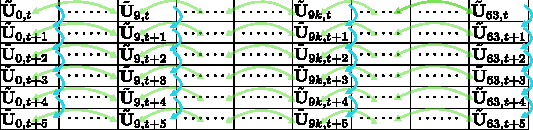
\includegraphics[width=0.5\textwidth]{images/table.pdf}
\caption{TX obtains feedback for $\{9k, k \in \{0,1,\ldots,7\}$ subcarriers, and uses $\tilde{\bU}_{i,t-1}$ to obtain $\tilde{\bU}_{i,t}$ using \eqref{pred_op} (cyan). For each time instant, TX uses Cayley method  \eqref{eqn:cayley_i1_i2} to interpolate $\tilde{\bU}_{i,t}$ at $i\neq\{9k\}$ non fed back subcarriers (green)}
\label{table}
\vspace{5pt}
\end{figure}

\subsection{Quantization error, BER and Achievable Rate Results}
\label{res}{}
% To mitigate errors in prediction upon the presence of randomly appearing drastic events in wireless channels, such as sudden interferences and dynamic environments, only 100 channel evolutions are considered for the simulations, and the algorithm is re-starte.
\noindent To ensure that the simulation results hold in general for the chosen IEEE Pedestrian A channel profile, we perform averaging over 100 independent channel realizations, each realization further evolved over 100 time instances as per the chosen doppler. Therefore, the quantization error, BER and achievable rate results are averaged over 10000 channel instances. From Fig. \ref{qtiz_err} it is evident that the RC framework is able to reduce the quantization error below what was obtained from the existing temporal correlations based predictive quantizer in \cite{6891198}. 
\begin{figure}
\centering
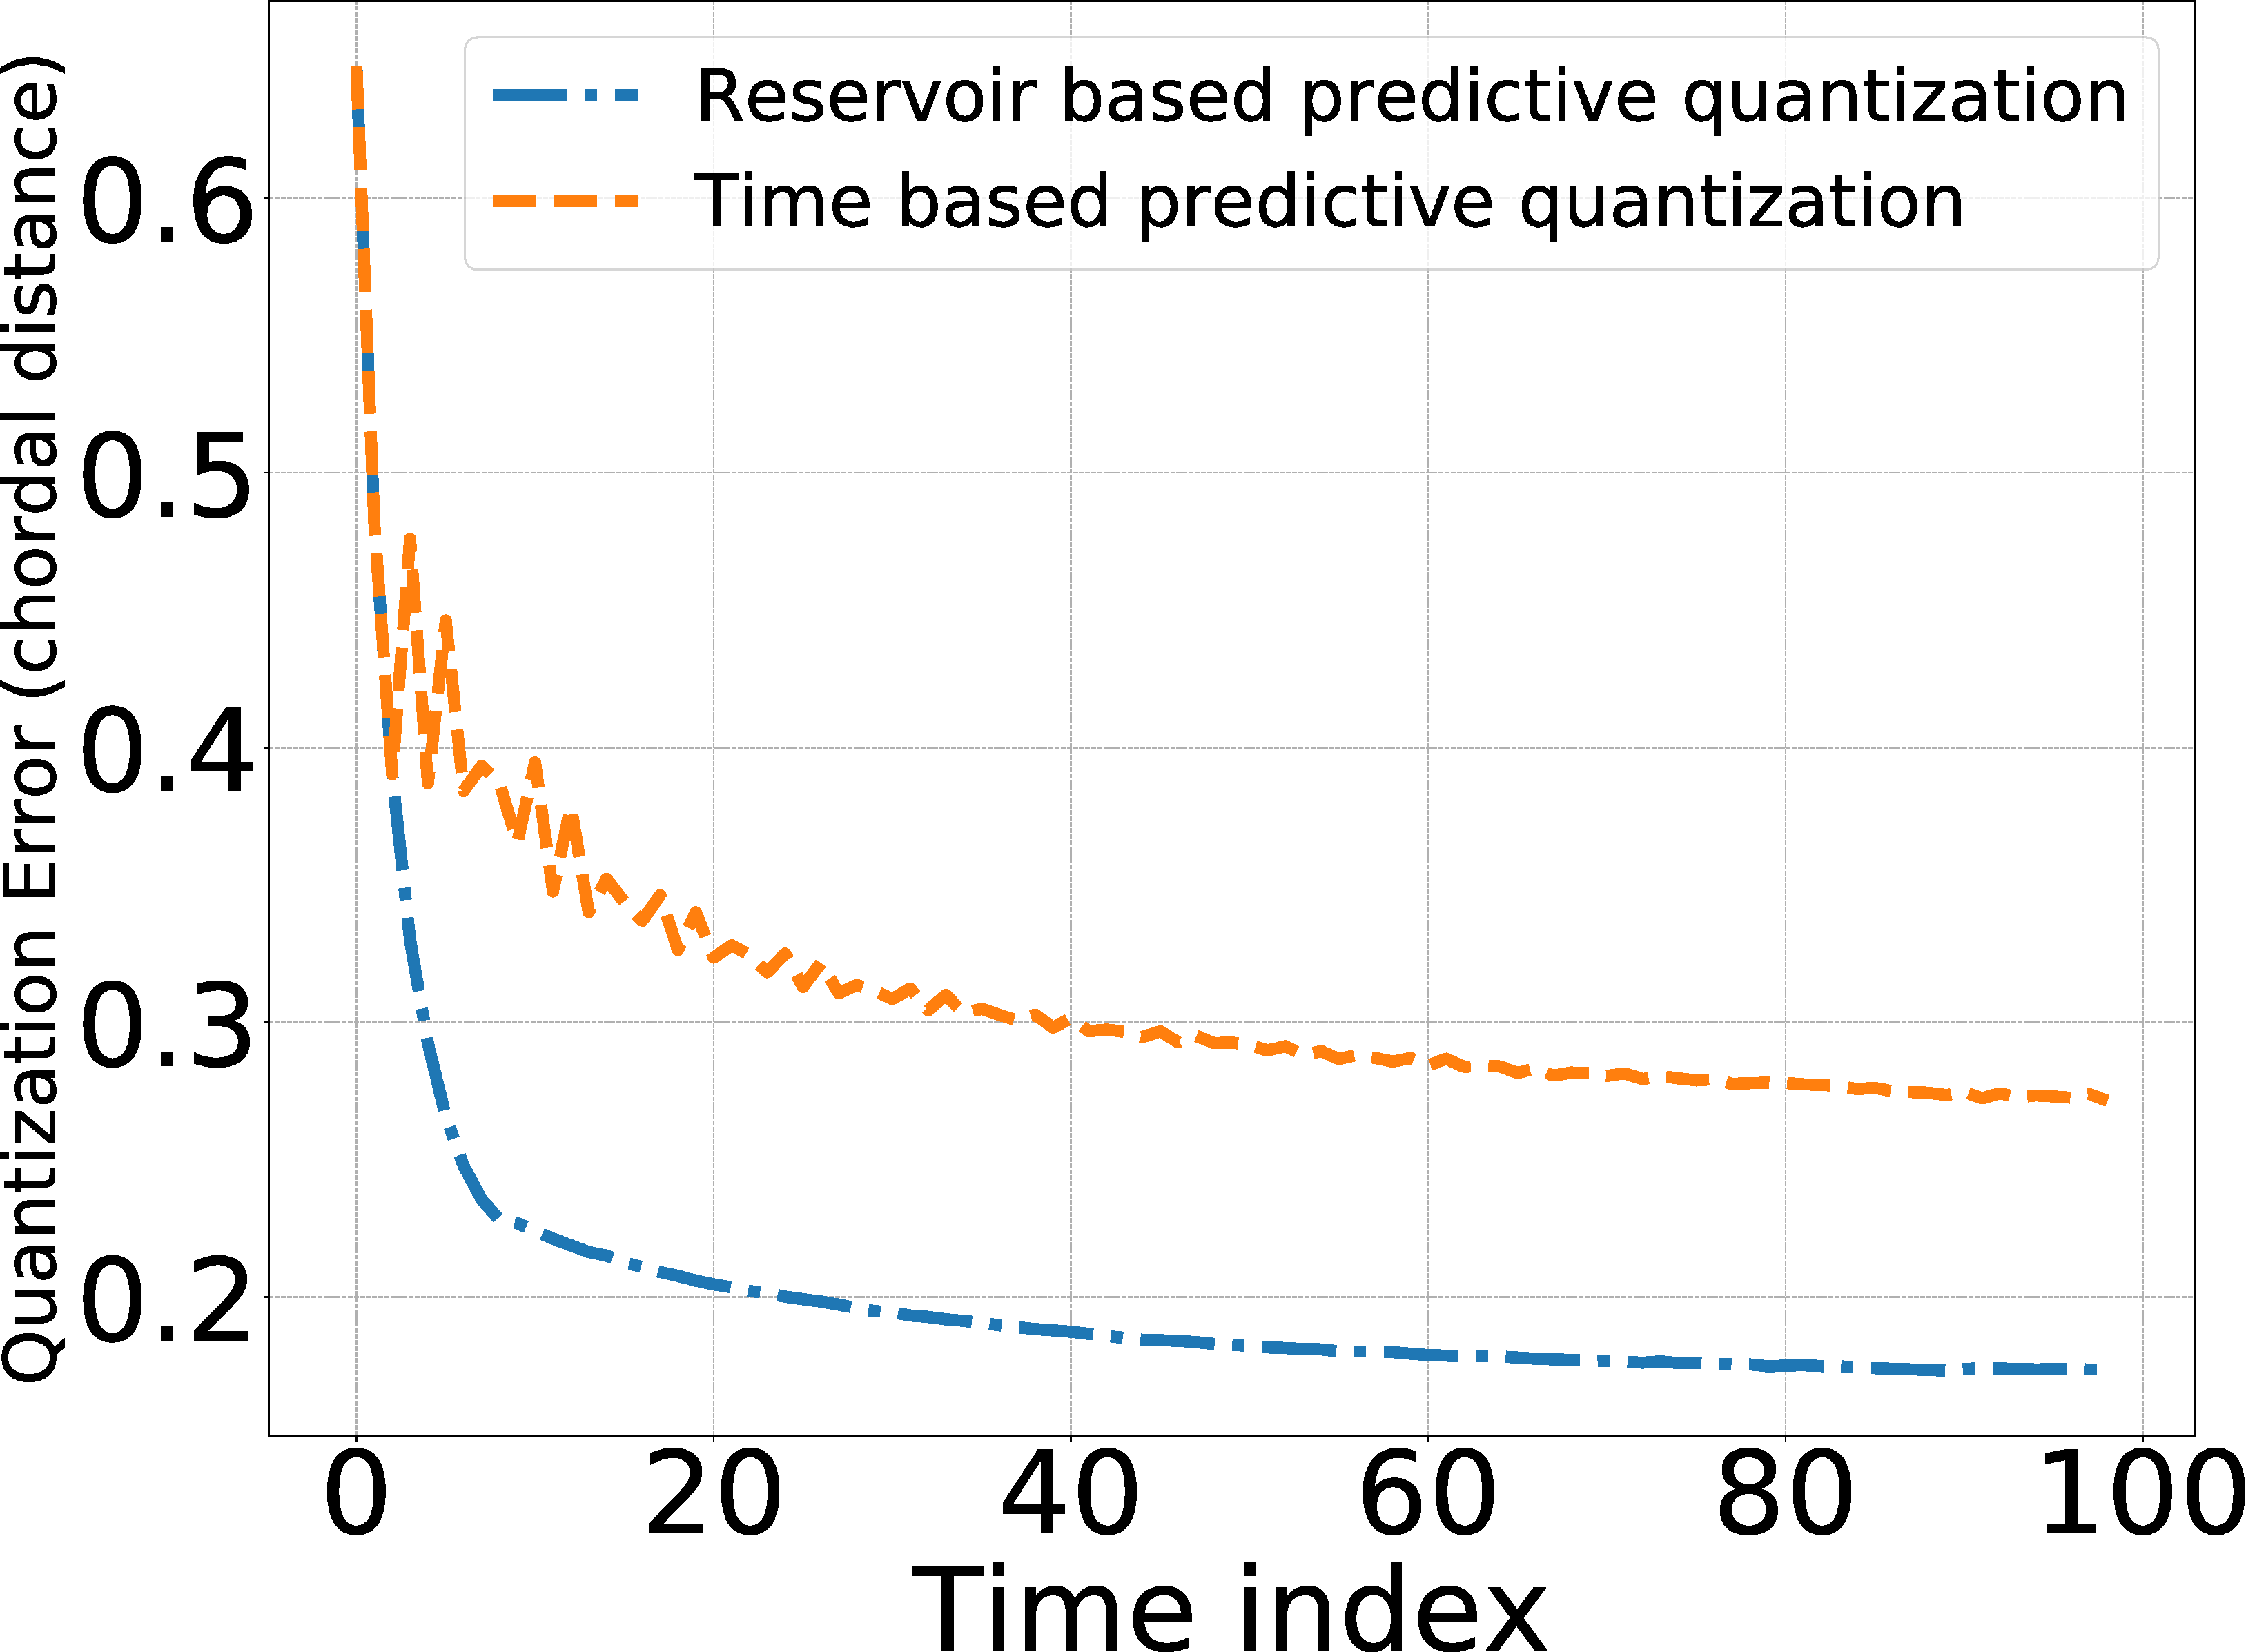
\includegraphics[width=0.35\textwidth]{images/qtizErr.pdf}
\caption{Quantization error in terms of chordal distance to the actual precoder $\bU_{\{9k\},t}$ observed at the receiver, from the quantized estimate $\tilde{\bU}_{\{9k\},t}$}
\label{qtiz_err}
\end{figure}

Observe from Fig. \ref{BER} that RC framework improves the BER performance substantially in the high SNR region. In the low SNR region, past work \cite{6891198} comes close to the lower bound curve (perfect estimates of 8 $\bU_{\{9k\},t}$ available at the transmitter), and hence, RC framework is not able to further improve the performance. However, for the high SNR region, there is considerable gap between the lower bound curve and BER curve by past work, and the RC framework BER curve lies in between the two, with improvements in $\frac{\text{E}_\text{b}}{\text{N}_0}$ greater than 5 dB at BERs lower than $\sim 10^{-6}$.  
% We simulate (uncoded QPSK) BER performance for all the 64 subcarriers' precoders obtained after interpolation ($\tilde{\bU}_{i\neq\{9k\},t}$) and quantization ($\tilde{\bU}_{\{9k\},t}$). Observe from Fig. \ref{BER} that RC framework is able to achieve substantial improvements in $\text{E}_\text{b}\text{N}_0$ levels at $\text{BER}\leq 10^{-4}$. Particularly, for $\text{BER}=10^{-5}$ we observe around $5$ dB improvement.  We hypothesize that the key reason for the improved performance for both quantization error and BER in the RC approach, is the fact that $f_P,q_P$ are coupled via the backward pass framework (explained towards the end of Section 2). 
% Also, observe from Fig. \ref{BER} that the proposed framework BER curve (yellow) comes very close to the ideal $8$ feedback curve (green). This can be explained due to the fact that the semi-unitary precoder basically rotates the data vector via its matrix transformation. For QPSK, we get some reasonable error margin for this rotation, which becomes more stringent as the simulated BER is reduced. Hence, we match the ideal curve for high BER region, and for low BER region, as the margin of error reduces, the curves diverge.
For simulating the achievable rate, we quantize the sigma values ($\Sigma_{i,t}$ from SVD of $\bH_{i,t}$) using a 2 bit $k$-means vector quantizer, and feed them back to the transmitter for fed back subcarriers. For non-fed back subcarriers, they are interpolated via a simple convex combination interpolation method as in \cite{Gupt1905:Predictive}. Observe from Fig. \ref{achievrate} that the RC framework offers improvement in achievable rate for $f_DT_s=10^{-4}$. Since the temporal variations for $f_DT_s=10^{-2}, 10^{-1}$ are higher, the RC framework has to learn a faster-varying function, and hence the degradation in performance. 
% However, it still matches the performance of the predictive quantizer in \cite{6891198} for $f_DT_s=10^{-2}$ and performs slightly better for $f_DT_s=10^{-1}$.
\vspace{-3pt}

\begin{figure}
\centering
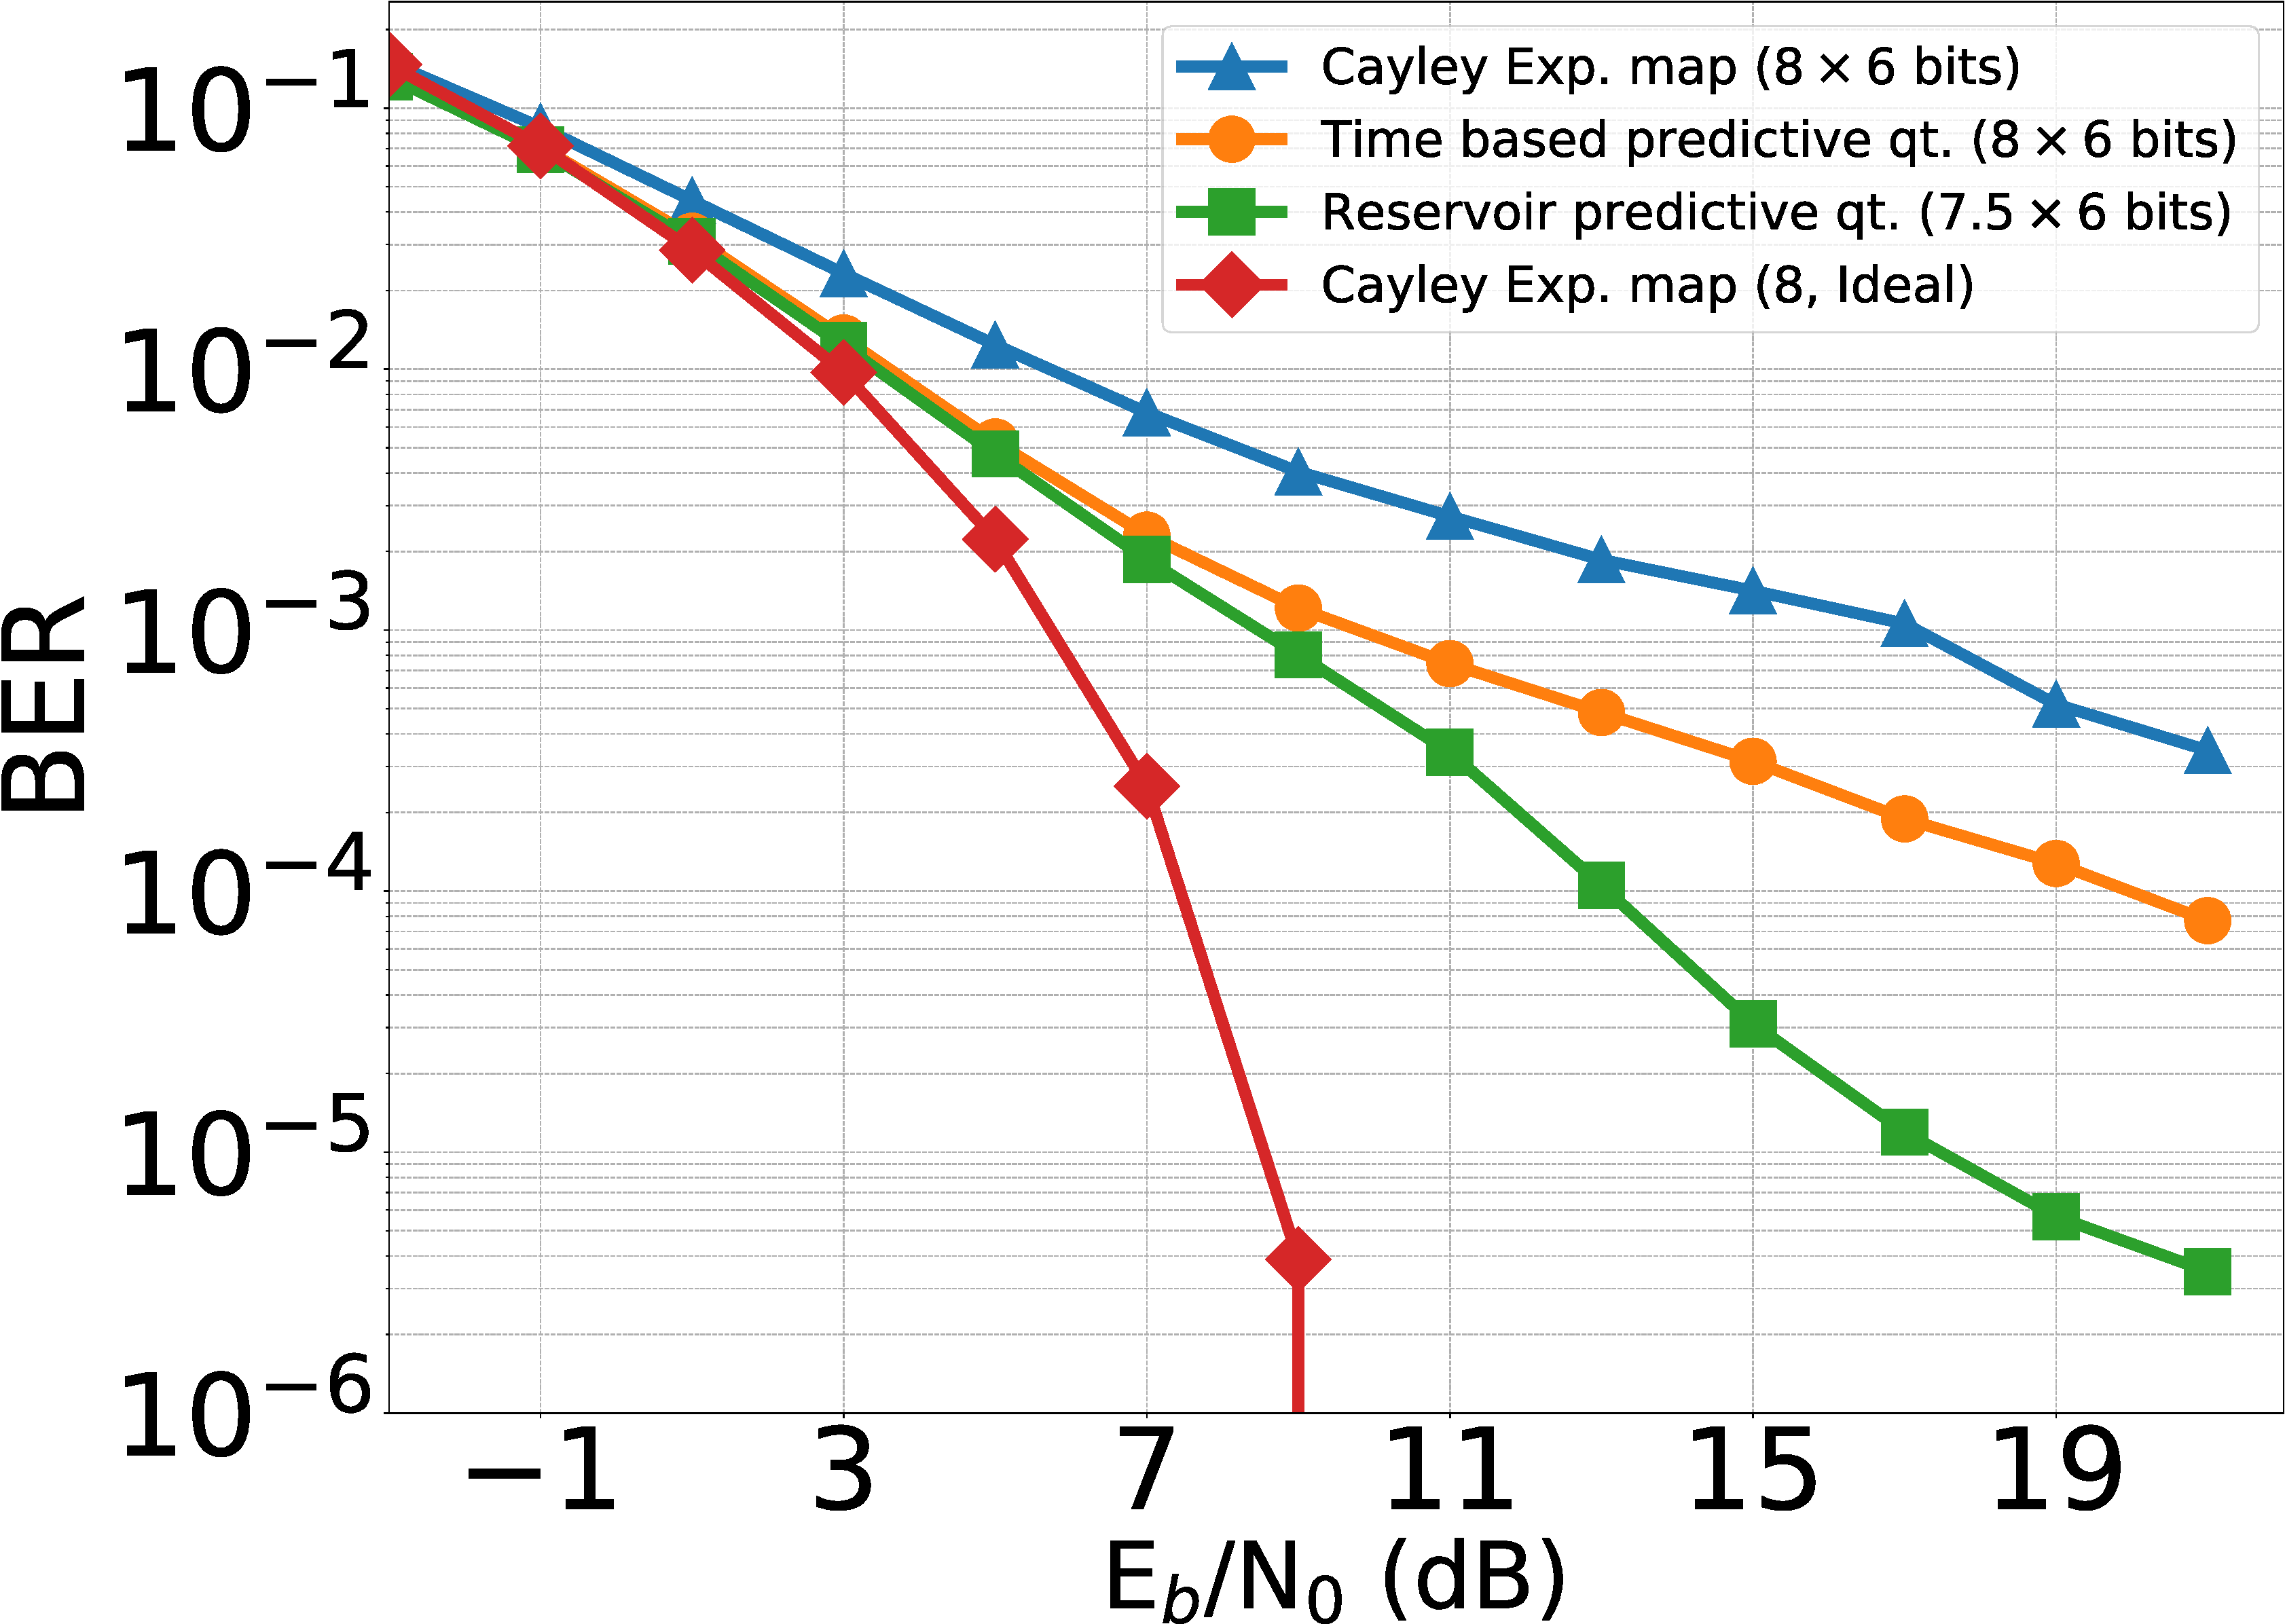
\includegraphics[width=0.35\textwidth]{images/BER_res.pdf}
\vspace{-5pt}
\caption{BER results: Here, red curve is the most ideal case considering exact $\bU_{i,t}$ for all 64 subcarriers, at each time instant are available at the transmitter. The \{green/yellow/blue\} curves corresponds to the case in which \{$\bU_{9k,t}$/$\tilde{\bU}_{9k,t}$ from reservoir method/$\tilde{\bU}_{9k,t}$ from \cite{6891198}\} is available for each time instant, and non fed back precoders are interpolated via Cayley method. Observe that the proposed framework BER curve provides significant improvement in $\text{E}_\text{b}\text{N}_0$ levels over \cite{6891198}}
\vspace{5pt}
\label{BER}
\end{figure}

\begin{figure}
\centering
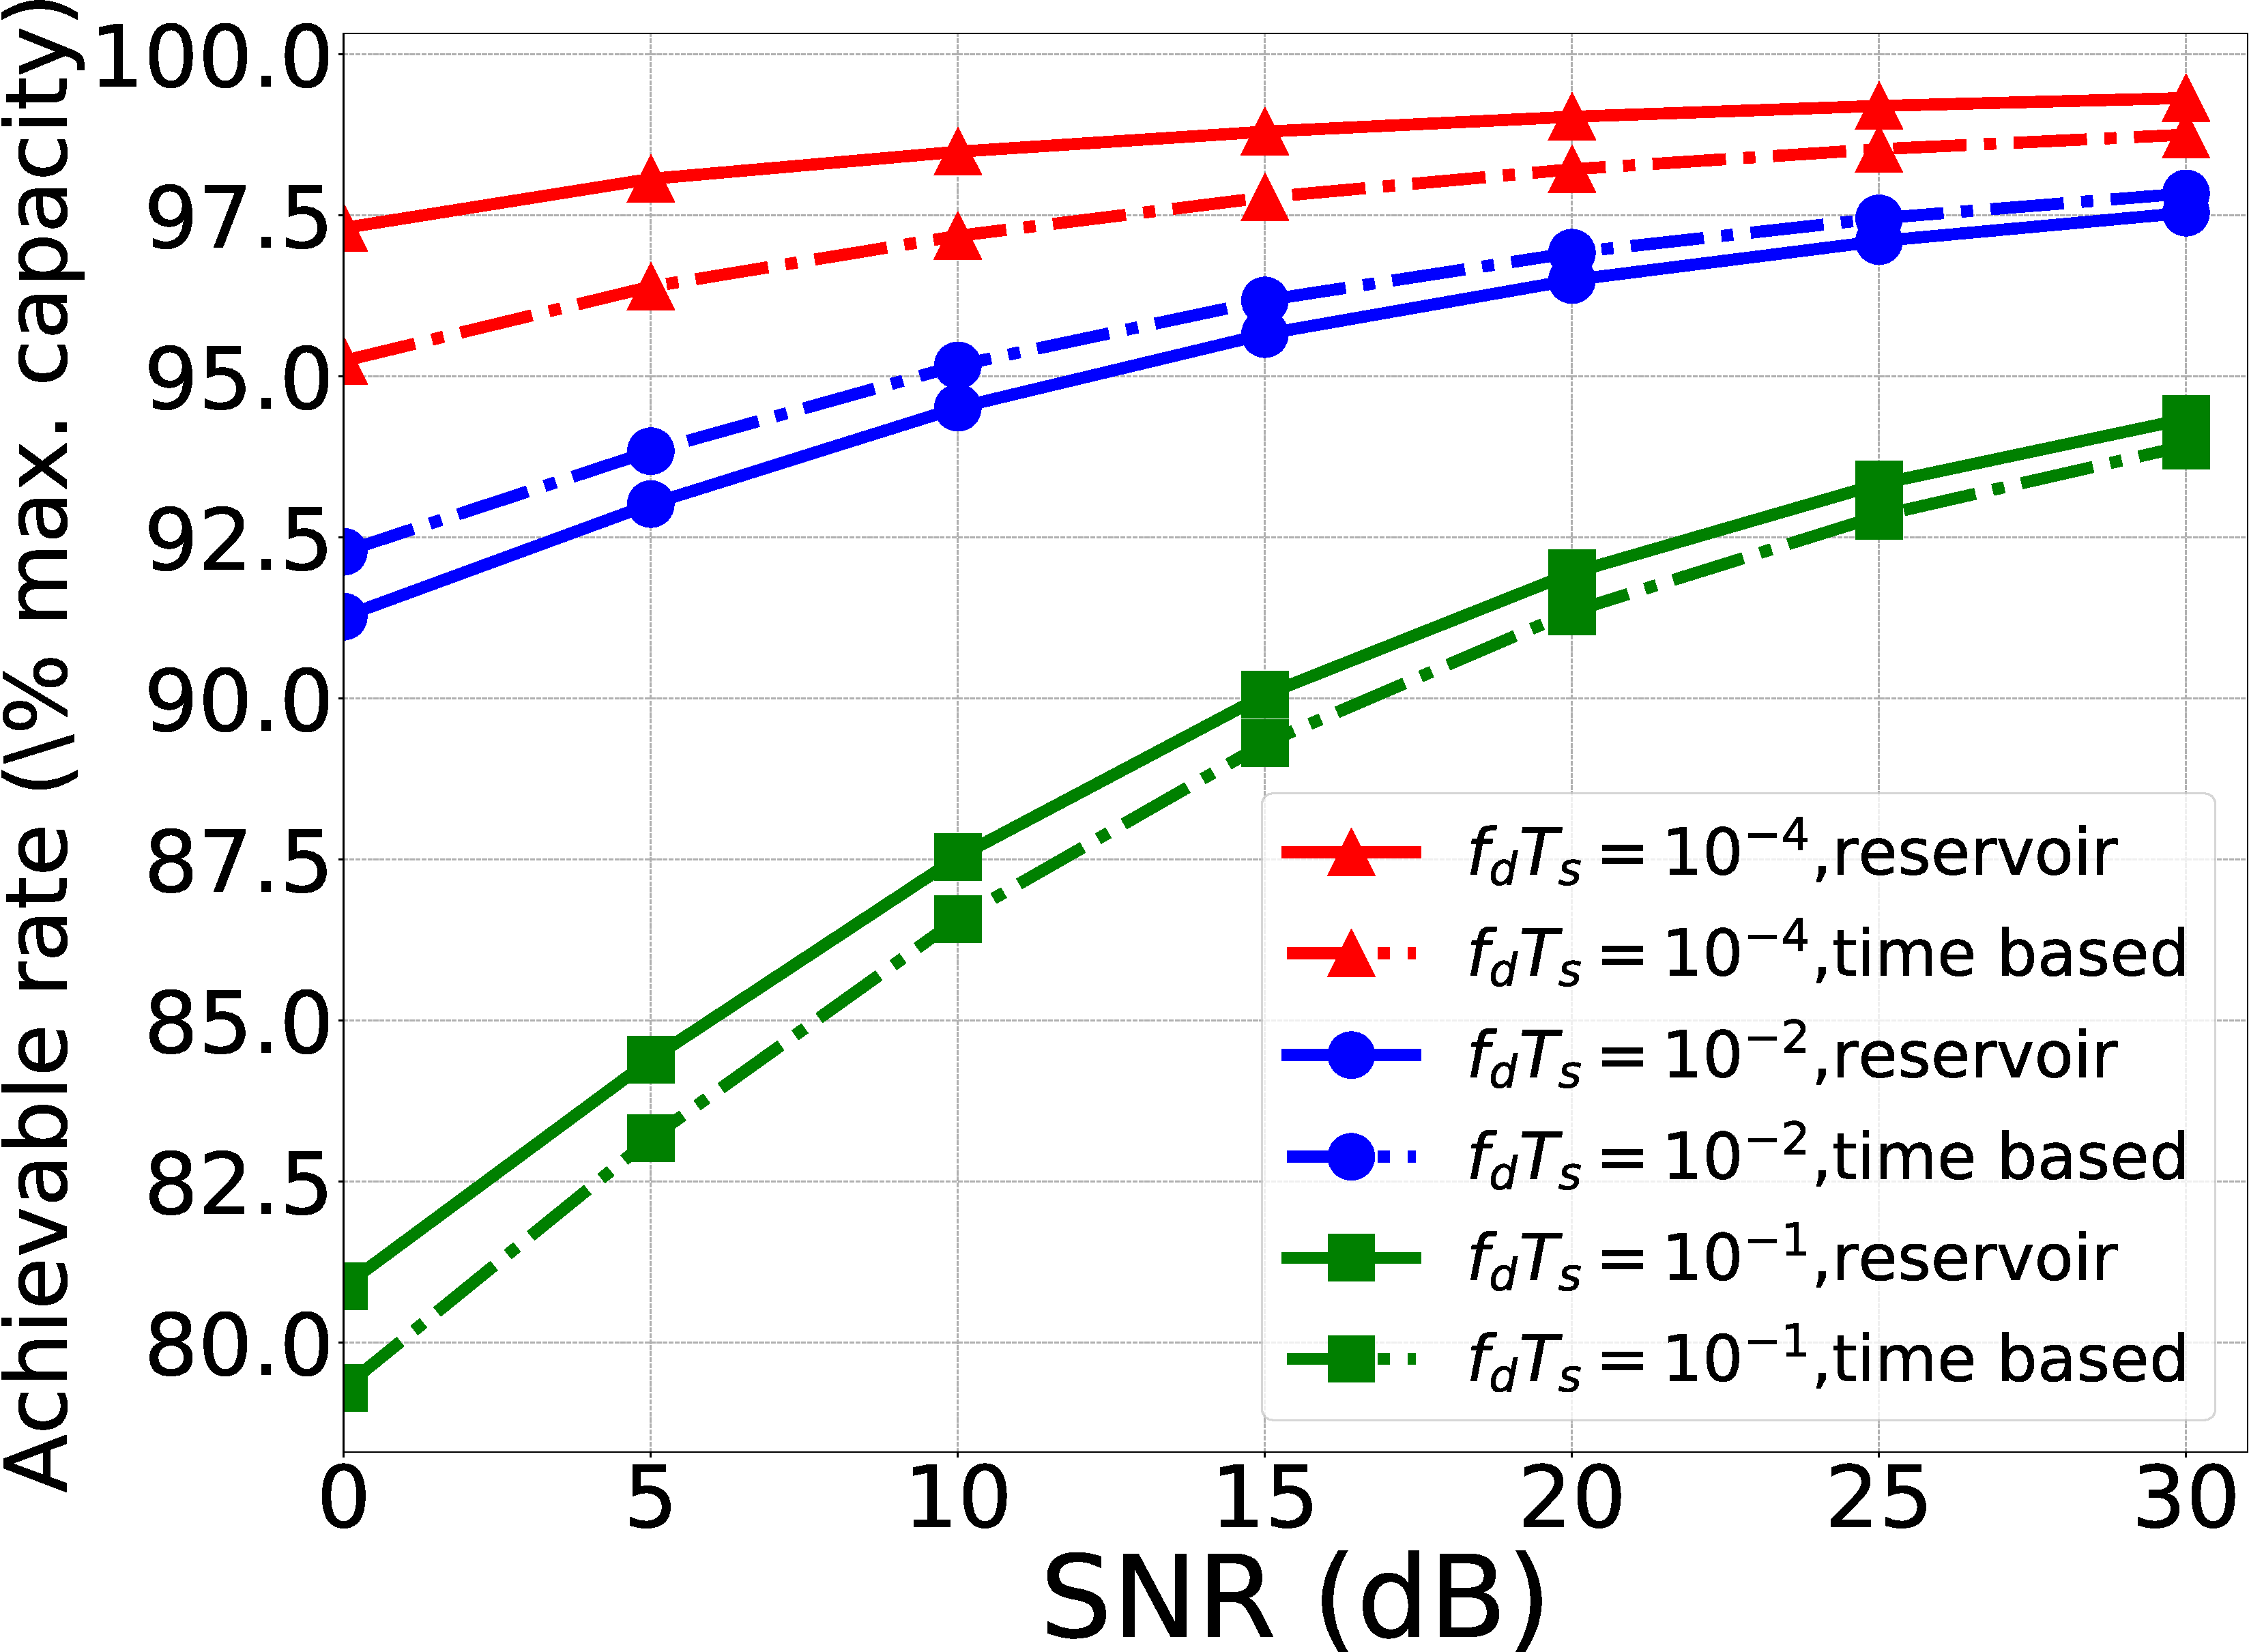
\includegraphics[width=0.35\textwidth]{images/hopRate.pdf}
\vspace{-5pt}
\caption{Achievable Rate results: Here, the results are presented as a percentage of the ideal rate obtained when the transmitter has full CSI, viz. the accurate(unquantized) $\bU_{i,t}$ for each subcarrier at each time instant. For both reservoir method, and Stiefel manifold method \cite{6891198}, 8 precoders are fed back similar to the setting for BER results (Fig. \ref{BER})}
\label{achievrate}
\vspace{-10pt}
\end{figure}
%Qtisn error with 1000 chan evols
%Qtisn error with 100 chan evols
%BER
%Achievable rat

\section{Conclusions and Future Work}
\label{section5}

We have presented a reservoir computing framework for predictive quantization of MIMO precoders by exploiting temporal correlations.
Simulations reveal significant improvement in quantization error, BER, and achievable rate.
The novelty that enables these improvements is the training method for the reservoir framework, which refines the predicted coarse estimates as the reservoir evolves.
Our results have been obtained by exploiting only temporal correlations for predictive quantization, and can potentially improve if frequency correlations are also exploited simultaneously..
Future work would focus on better reservoir frameworks, and a detailed analysis of impact on performance caused by choice of different reservoir parameters like $\bA,\text{tanh}(\cdot),$ and $D_{\text{resv}}$.
\vspace{-4pt}

% \section{Acknowledgment}
% % \label {section6}
% % \input{sections/6_section.tex}
% Parts of this work was supported by the Bharti Centre for Communication in
% IIT Bombay, and the Visvesvaraya
% PhD Scheme of Ministry of Electronics \& Information Technology,
% Government of India, being implemented by Digital India Corporation.


\renewcommand{\bibfont}{\footnotesize}
\bibliography{IEEEabrv,main}
\bibliographystyle{IEEEtran}
\end{document}

% Remove the first para of FSM. State what r1,r2,d,\theta are in the FSM model states themselves. As a concluding statement of STAT-2 state that using the
% inherit geometery of the problem, we get AoA
